\documentclass[acmsmall,screen,review,anonymous]{acmart}
\usepackage{amsmath}
\usepackage{algorithm}
\usepackage{algorithmicx}
\usepackage{algpseudocode}
\usepackage{tabularx}
\newcommand{\E}{\mathbb{E}}
\newcommand{\I}{\mathbb{I}}
\newtheorem{proposition}{Proposition}
\newtheorem{definition}{Definition}
\newtheorem{assumption}{Assumption}
\makeatletter
\providecommand*{\toclevel@algorithm}{1}
\providecommand*{\theHalgorithm}{\thealgorithm}
\makeatother
\citestyle{acmnumeric}
% Retain the default ACM permission and reference-format blocks.
% Publication identifiers are unassigned at initial review.
\acmConference[FSE 2027]{ACM International Conference on the Foundations of Software Engineering}{12-16 July 2027}{Shenzhen, China}
\acmBooktitle{ACM International Conference on the Foundations of Software Engineering (FSE 2027), 12-16 July 2027, Shenzhen, China}
\acmYear{2027}
\copyrightyear{2027}
\acmDOI{}
\acmISBN{}
\begin{document}
\title[Hybrid-INoT]{Hybrid-INoT: a hybrid agent architecture with internal role segregation for engineering tasks under long shared context}
\begin{abstract}
External multi-agent orchestration repeatedly transmits shared context to separate large-language-model roles, increasing token usage. We propose \textbf{Hybrid-INoT}, a hybrid architecture in which the \textit{planner--worker--critic--self-check} cycle is executed inside one model call, while tool actions, verification, and context compression remain external. We define its operational model, routing function, and analytical conditions for token and economic efficiency. A reproducible evaluation uses HumanEval and a controlled task set. In a real Gemini~3.1~Pro Preview API pilot ($n=5$ tasks per context length), Hybrid-INoT reduced mean token consumption relative to Classical-MAS by 55.6--88.9\% as target context grew from 256 to 16,384 tokens; an independent Gemini~3.1~Flash-Lite run ($n=20$, seed 42) yielded 49.6--90.3\% savings. In the latter run, the paired $U_{\mathrm{tok}}$ gain was significant at all four context lengths after Holm--Bonferroni correction ($p=1.91\cdot10^{-6}$). However, pass@1 was 1.0 for both architectures, so the stated quality non-inferiority margin was not statistically established. The small-model profitability condition held in the HumanEval pilot but not in the approximate SWE-bench Lite protocol. An analytical extrapolation of observed Pro API costs gives \$429.96 savings per 10,000 tasks under an equal mixture of four context lengths (95\% bootstrap CI \$267.06--\$617.17); this is not a full-TCO estimate. The evidence therefore supports token efficiency in the studied range but does not establish quality preservation, transfer to real repositories, or lower total cost of ownership.
\end{abstract}
\ccsdesc[500]{Software and its engineering~Automatic programming}
\ccsdesc[300]{Computing methodologies~Multi-agent systems}
\keywords{Large language models, agent systems, Introspection of Thought, token efficiency, inference economics, HumanEval, reproducible experiment}
\maketitle
\section{Introduction}\label{sec:intro}

A modern software-engineering agent must successively understand the task specification, retrieve the relevant context from a repository, and construct a change that can then be checked by tests or static analysis. In practice, these functions are often distributed across several roles: one role builds a plan, another proposes a solution, a third critiques the intermediate result, and a fourth runs external verification. This decomposition is conceptually convenient, but it becomes expensive when all roles are forced to reread the same long context.

This paper focuses precisely on that setting: tasks in which the code, documentation, compiler messages, and execution logs are shared across all roles. We are interested not only in the final solution quality but also in the cost of the chosen orchestration scheme in tokens, response time, and monetary spending. The article therefore compares classical external multi-agent organization with a hybrid scheme in which part of the role discussion is moved inside a single model call.

\subsection{The problem of repeated context transmission and its practical significance}

In agent systems built on large language models, a typical configuration is external multi-agent orchestration (\textrm{Classical-MAS}): separate processes or calls implement the planner, worker, critic, and tester roles \cite{hong2023metagpt,qian2023chatdev,guo2024survey}. In software-engineering tasks, where several roles read the same long fragments of code, logs, and documentation, this scheme has a structural defect: \emph{each role receives the shared context $\mathcal{C}_0$ anew}, and additional coordination messages circulate between roles. In token-budget terms, this yields the term
\[
D_{\text{ctx}}+H_{\text{coord}} \;\;\in\;\; \Theta(|\mathcal{A}|\cdot|\mathcal{C}_0|)+\Theta(|\mathcal{A}|^2\cdot\bar{h}),
\]
where $|\mathcal{A}|$ is the number of roles and $\bar{h}$ is the average coordination-message length. In our API pilot, this structural effect was observed directly. At a target context of 16,384 tokens, \textrm{Classical-MAS} used 59,631 tokens per task on average, of which 57,485 (96.4\%) were input tokens; \textrm{Hybrid-INoT} used 6,608 tokens. Per-case cost was \$0.14072 and \$0.02949, respectively, at the recorded Gemini~3.1~Pro Preview prices~\cite{openrouterpro2026}. These values concern the first five HumanEval tasks and must not be generalized to a different task distribution without measurement.

The problem is therefore quantitatively observable: in the studied long-context regime, repeated input transmission produced an approximately ninefold difference in total tokens between B2 and B3. The remainder of the paper separates the analytical model from empirical evidence and restricts claims to completed pilots.

\subsection{Existing approaches and their limitations}

The open literature contains three related lines of work: (i)~single-model in-context self-critique, such as Self-Refine~\cite{madaan2023selfrefine} and Reflexion~\cite{shinn2023reflexion}; (ii)~alternation between reasoning and action inside one agent, such as ReAct~\cite{yao2022react} and SWE-agent~\cite{yang2024sweagent}; and (iii)~external role decomposition into separate calls, such as MetaGPT~\cite{hong2023metagpt} and ChatDev~\cite{qian2023chatdev}. None of these works defines an \emph{operationally distinct} intermediate configuration in which (a)~the shared context is preserved inside one call without duplication, (b)~role segregation remains sufficient for critical examination, and (c)~only operations with externally verifiable signals, such as tests, static analysis, and tool calls, remain external. The literature also lacks a formal condition under which such a hybrid dominates a purely external \textrm{Classical-MAS} scheme in expected token consumption.

\subsection{Main results and contribution}

The paper delivers the following results:
\begin{enumerate}
\item[\textbf{C1.}] An operational definition of Hybrid-INoT with an explicit state signature, the \textnormal{\texttt{RouteMode}} routing function, and a termination condition for the internal role cycle (§\ref{sec:method}).
\item[\textbf{C2.}] Proposition~\ref{prop:inot-vs-mas}, which states the token advantage of Hybrid-INoT over Classical-MAS in expectation when the shared context is sufficiently long, and proves it by an explicit token accounting under stated assumptions (§\ref{sec:analysis}).
\item[\textbf{C3.}] Inequality~\eqref{eq:small-model-condition}, which gives the profitability condition for a small self-check model (§\ref{sec:analysis}).
\item[\textbf{C4.}] A system of metrics for token efficiency, monetary cost, and code maintainability with a justified aggregation form (§\ref{sec:metrics}).
\item[\textbf{C5.}] A reproducible real-API evaluation covering context-length scaling, ablations, the small-model check, and an E6 cross-model sensitivity analysis (§\ref{sec:eval}).
\item[\textbf{C6.}] Evidence-aligned hypothesis verdicts: support for the token component of H1 in the Flash-Lite run, partial support for H2 only on HumanEval, and no support for H3 in the direct architectural comparison (§\ref{sec:eval}).
\end{enumerate}

\noindent The harness, configurations, raw results, and figure-generation script are linked to an immutable research commit (§\ref{sec:eval}).

\section{Related work and distinction of the proposed approach}\label{sec:related}

\subsection{From chain-of-thought to internal role debate}

Wei et al.~\cite{wei2022cot} show that explicit verbalization of intermediate reasoning steps can improve solution quality on tasks that require several connected logical transitions. In this context, intermediate steps are textual fragments by which the model decomposes a complex inference into a sequence of local subproblems, while quality refers to the final success of solving the target task. The \textrm{Self-Refine} approach \cite{madaan2023selfrefine} formalizes a ``generator--feedback--revision'' cycle inside a single model; \textrm{Reflexion} \cite{shinn2023reflexion} supplements such a scheme with reflective memory, whereas \textrm{ReAct} \cite{yao2022react} couples internal reasoning with external actions and tools. Sun and Zeng \cite{sun2025inot} describe \textit{Introspection of Thought} (INoT) as a structured internal debate among several roles. At the same time, Turpin et al.~\cite{turpin2023unfaithful} show that intermediate chain-of-thought text should not be interpreted as a faithful description of the hidden computational process. Accordingly, in the present paper introspection is treated primarily as a computational mechanism for candidate selection, critique, and selective rerun rather than as a literal window into the latent state of the model.

\subsection{Multi-agent systems for software engineering}

Weiss \cite{weiss1999} and Wooldridge \cite{wooldridge2009} provide the theoretical framework for MAS. MetaGPT \cite{hong2023metagpt} and ChatDev \cite{qian2023chatdev} transfer this framework into the context of large language models: roles are implemented as separate calls, each receiving its own copy of the context. Survey work identifies two key limitations of Classical-MAS: error propagation along the chain and the growth of coordination cost \cite{guo2024survey,qian2024scaling}. SWE-bench and SWE-agent \cite{jimenez2023swebench,yang2024sweagent} further show that practical software-engineering automation requires long context and iterative editing, which makes the retransmission problem $D_{\text{ctx}}$ even more acute.

\subsection{Context compression and external verification}

LongLLMLingua and LLMLingua-2 \cite{jiang2023longllmlingua,pan2024llmlingua2} demonstrate that prompt compression can preserve or even improve quality under long context while lowering cost. Jia et al.~\cite{jia2026compression} apply this logic directly to code. For code self-check, linguistic reflection alone is insufficient: external observable signals are required, namely tests, static analysis, and compiler feedback~\cite{bi2024cocogen,su2025static,sepidband2025complexity}.

\subsection{Comparison of Hybrid-INoT with prior approaches}\label{subsec:distinction}

To systematize the differences among the architectures under discussion, we distinguish five features: context organization, the structure of role interaction, the verification mechanism, the way the execution mode is chosen, and the stopping condition.

\begin{table}[htbp]
\caption{Comparison of Hybrid-INoT with adjacent architectural classes}
\label{tab:distinction}
\centering
\begingroup
\begin{tabularx}{\textwidth}{@{}>{\raggedright\arraybackslash}p{2.8cm}>{\raggedright\arraybackslash}X>{\raggedright\arraybackslash}X>{\raggedright\arraybackslash}X@{}}
\toprule
Feature & Self-Refine / Reflexion & MetaGPT / ChatDev & Hybrid-INoT \\
\midrule
Context organization & One shared context without explicit role separation. & A separate copy of the shared context is created for each role. & One shared context is preserved inside a model call and shared among the internal roles. \\
Role interaction & Self-critique is embedded in a single-model loop. & Roles are separated into distinct calls and exchange messages. & Planning, generation, and critique are executed as internal roles within one cycle. \\
Solution verification & Predominantly linguistic self-evaluation. & Predominantly role-based linguistic checking; external verification depends on the implementation. & The final candidate must pass external tool-based verification; linguistic critique is used as an intermediate filter. \\
Mode selection & Fixed by the method architecture. & Fixed by the method architecture. & Set by an explicit routing function that switches between internal and external modes. \\
Stopping condition & A fixed number of iterations or an episodic stopping rule. & Completion of the role pipeline or agreement among roles. & Stop after successful external verification or after the iteration limit is reached. \\
\bottomrule
\end{tabularx}
\endgroup
\end{table}

Table~\ref{tab:distinction} shows that individual components of the proposed scheme appear in earlier work, but it is precisely their combination inside a single internal role cycle, supplemented by external tool-based verification and explicit routing, that constitutes the Hybrid-INoT architecture.

\section{Formal problem statement}\label{sec:problem}

\subsection{Task}

Let $\mathcal{X}$ denote the set of textual task specifications, $\mathcal{C}$ the set of finite sequences of contextual artifacts (code files, documentation fragments, and execution logs), and $\mathcal{Y}$ the set of candidate solutions representable as textual artifacts and amenable to external verification. Let $(\Omega,\mathcal{F},\mathbb{P})$ be the probability space induced by stochastic model generation, seed choice, and nondeterminism in external tool calls.

\begin{definition}[Agentic engineering task]\label{def:task}
An agentic engineering task is the tuple $(x,\mathcal{C}_0,\mathcal{Z},\mathcal{V})$, where $x\in\mathcal{X}$ is a textual task description; $\mathcal{C}_0\in\mathcal{C}$ is the initial task context, including code, documentation, and execution logs; $\mathcal{Z}$ is a finite set of permitted external tools; and $\mathcal{V}:\mathcal{Y}\to\{0,1\}$ is an externally verifiable success function, for example, the execution of a test suite.
\end{definition}

The agent strategy induces a random output $Y:\Omega\to\mathcal{Y}$. At the same time, random variables $T:\Omega\to\mathbb{R}_{\ge 0}$, $C_{\text{inf}}:\Omega\to\mathbb{R}_{\ge 0}$, and $\ell:\Omega\to\mathbb{R}_{\ge 0}$ are defined, representing, respectively, the total token consumption, the monetary inference cost, and the latency of solving one task. The goal of the agent is to maximize $\E[\mathcal{V}(Y)]$ under the budget constraints $\E[T]\le B$, $\E[C_{\text{inf}}]\le B_\$$, and $\E[\ell]\le B_\ell$.

\subsubsection*{Main notation}
\begin{description}
\item[$\mathcal{C}_0$] --- the initial shared task context; $|\mathcal{C}_0|$ is its token length.
\item[$\hat{\mathcal{C}}$] --- the compressed version of the initial context used in the internal cycle.
\item[$\mathcal{A}$] --- the set of external roles in the \textrm{Classical-MAS} scheme; $|\mathcal{A}|$ is the number of such roles.
\item[$Y$] --- the random output of the agent with values in $\mathcal{Y}$; $y\in\mathcal{Y}$ is an individual candidate solution.
\item[$K$] --- the number of candidates generated by the role $r_{\text{work}}$ in one iteration of the internal cycle.
\item[$T$] --- the random variable of total token consumption for one task; $\E[T]$ is taken with respect to the distribution defined on $(\Omega,\mathcal{F},\mathbb{P})$.
\item[$U_{\text{tok}}$] --- the token-efficiency measure defined as the ratio of final solution quality to total token consumption.
\item[$\tau^\star$] --- the threshold initial-context length beyond which \textrm{Hybrid-INoT} has an expected token advantage.
\item[$\delta_{H1}$] --- the minimal practically relevant gain in $U_{\text{tok}}$ used in Hypothesis~H1.
\item[$C_{\text{check}}^S$] --- the cost of the preliminary check performed by the small model.
\item[$C_{\text{rerun}}^L$] --- the cost of rerunning the large model.
\item[$\rho_0,\rho_1$] --- the probabilities of an expensive rerun without and with the preliminary check, respectively.
\end{description}

\subsection{Research hypotheses}

\begin{description}
\item[]\textbf{H1} (advantage under long context).\quad There exists a threshold initial-context length $\tau^\star$ such that for $|\mathcal{C}_0|>\tau^\star$, \textrm{Hybrid-INoT} yields at least a $\delta_{H1}=15\%$ increase in $U_{\text{tok}}$ relative to \textrm{Classical-MAS}, while pass@1 degrades by no more than 2 percentage points.\par\emph{Verification:} E3 (§\ref{subsec:e3}) with paired Wilcoxon tests, 95\% bootstrap confidence intervals, and Holm--Bonferroni correction.
\item[]\textbf{H2} (economic justification of the small self-check model).\quad There exists a regime in which a small-model preliminary check reduces expensive reruns enough for $C_{\text{check}}^S<(\rho_0-\rho_1)C_{\text{rerun}}^L$.\par\emph{Verification:} E4 (§\ref{subsec:e4}) on 20 HumanEval tasks and 20 approximate SWE-bench Lite cases.
\item[]\textbf{H3} (boundary of applicability).\quad On tasks with genuinely independent subtasks and parallel tools, the response-time advantage of Hybrid-INoT vanishes or becomes negative.\par\emph{Verification:} an architectural comparison on five tasks and a separate controlled serial/parallel tool microbenchmark in E2c (§\ref{subsec:e2}).
\end{description}

When testing H1, the base model, tools, external verification, task set, seed, temperature, and prompts are held fixed; only orchestration changes. The threshold $\delta_{H1}=15\%$ is treated as the minimum practically meaningful effect. Observed savings do not replace evaluation of the complete H1 criterion.

\section{Method: Hybrid-INoT}\label{sec:method}

\subsection{States and role signatures}

Define the system state as $\sigma=(x,\hat{\mathcal{C}},\mathcal{H},i,b)$, where $\hat{\mathcal{C}}$ is the compressed context, $\mathcal{H}$ is the history of iterations, $i\in\{0,\dots,I\}$ is the iteration counter, and $b\in\mathbb{N}$ is the remaining token budget.

Let $\Pi$ be the space of plans, and let $K\in\mathbb{N}$ denote the number of candidates generated by the role $r_{\text{work}}$ in one iteration. Then each role is defined by a signature $r:\mathcal{S}_r^{\text{in}}\to\mathcal{S}_r^{\text{out}}$:
\begin{align*}
r_{\text{plan}} &:(x,\hat{\mathcal{C}},b)\mapsto \pi\in\Pi, \\
r_{\text{work}} &:(\pi,\hat{\mathcal{C}},K)\mapsto \mathbf{y}=(y_1,\dots,y_K)\in\mathcal{Y}^K, \\
r_{\text{crit}} &:(\mathbf{y},\hat{\mathcal{C}})\mapsto (s_1,\dots,s_K)\in[0,1]^K, \\
r_{\text{self}} &:(y\in\mathcal{Y})\mapsto (v,M)\in\{0,1\}\times[0,1].
\end{align*}
The roles $r_{\text{plan}},r_{\text{work}},r_{\text{crit}}$ are implemented as role prefixes inside \emph{one} large-model call over the shared $\hat{\mathcal{C}}$; the role $r_{\text{self}}$ is an external process running tests and static analysis.

\subsection{Routing function}

\begin{definition}[RouteMode]\label{def:routemode}
Let $\varphi_{\mathrm{tool}}(x)\in\{0,1\}$ indicate whether an external tool is mandatory, let $\varphi_{\mathrm{par}}(x)\in\{0,1\}$ indicate dominant subtask parallelism, and let $|\hat{\mathcal{C}}|$ be the length of the compressed context. Then
\[
\textnormal{\texttt{RouteMode}}(x,\hat{\mathcal{C}})=\begin{cases}\textnormal{\texttt{external}}, & \varphi_{\mathrm{tool}}(x)=1 \;\lor\; \varphi_{\mathrm{par}}(x)=1 \;\lor\; |\hat{\mathcal{C}}|<\tau^\star_{\mathrm{route}},\\ \textnormal{\texttt{internal}}, & \text{otherwise}.\end{cases}
\]
The parameters $\varphi_{\mathrm{tool}}$ and $\varphi_{\mathrm{par}}$ are determined by a separate classifier over $x$ (a lightweight instruction-based classifier in the base implementation). The threshold $\tau^\star_{\mathrm{route}}=1024$ tokens remains an engineering setting and must not be conflated with the left-censored research result $\tau^\star\le256$ from E3.
\end{definition}

\subsection{Internal cycle and termination condition}

\begin{algorithm}[htbp]
\caption{Hybrid-INoT: internal introspective cycle}\label{alg:main}
\begin{algorithmic}[1]
\Require task $x$, context $\mathcal{C}_0$, budget $B$, maximum number of iterations $I$, number of candidates $K$
\Ensure solution $y^\star$, flag $v^\star$, score $M^\star$
\State $\mathcal{C}\gets\textnormal{\texttt{PolicySanitize}}(x,\mathcal{C}_0)$
\State $\hat{\mathcal{C}}\gets\textnormal{\texttt{CompressIfNeeded}}(\mathcal{C})$ \Comment{Alg.~\ref{alg:compression}}
\State $m\gets\textnormal{\texttt{RouteMode}}(x,\hat{\mathcal{C}})$ \Comment{Def.~\ref{def:routemode}}
\If{$m=\textnormal{\texttt{external}}$} \Return \textnormal{\texttt{ExternalAgentWorkflow}}$(x,\hat{\mathcal{C}})$ \EndIf
\State $s^{\text{best}}\gets-\infty;\; y^{\text{best}}\gets\bot$
\For{$i=1$ to $I$}
 \State $\pi_i\gets r_{\text{plan}}(x,\hat{\mathcal{C}},B-\text{spent})$
 \State $\{y_{i,k}\}\gets r_{\text{work}}(\pi_i,\hat{\mathcal{C}},K)$
 \State $(s_{i,1},\dots,s_{i,K})\gets r_{\text{crit}}(\{y_{i,k}\},\hat{\mathcal{C}})$
 \State $k^\star\gets\arg\max_k s_{i,k};\; y_i\gets y_{i,k^\star}$
 \If{$s_{i,k^\star}>s^{\text{best}}$} $s^{\text{best}}\gets s_{i,k^\star};\; y^{\text{best}}\gets y_i$ \EndIf
\State $(v_i,M_i)\gets r_{\text{self}}(y_i)$ \Comment{external tests and static analysis}
 \If{$v_i=1$} \Return $(y_i,1,M_i)$ \EndIf
 \State $\hat{\mathcal{C}}\gets\textnormal{\texttt{UpdateContextWithFailures}}(\hat{\mathcal{C}},v_i)$
 \If{$\operatorname{stagnation}(s_{i,k^\star}-s_{i-1,k^\star})<\varepsilon$} \textbf{break} \Comment{see Prop.~\ref{prop:convergence}}\EndIf
\EndFor
\State \Return $(y^{\text{best}},0,M(y^{\text{best}}))$
\end{algorithmic}
\end{algorithm}

\begin{proposition}[Termination of the internal cycle]\label{prop:convergence}
Assume that each operation within one iteration of Algorithm~\ref{alg:main} terminates in finite time and that the number of iterations is bounded above by the parameter $I$. Then the algorithm terminates no later than after $I$ iterations: it either returns a solution immediately after a successful external check $v_i=1$, or stops earlier under the rule $\operatorname{stagnation}(s_{i,k^\star}-s_{i-1,k^\star})<\varepsilon$, or, after exhausting the iteration limit, returns the best candidate found.
\end{proposition}

\begin{proof}
The outer loop over the index $i$ contains at most $I$ passes. Each iteration consists of a finite sequence of steps: plan construction, generation of $K$ candidates, critical scoring, external verification, and context update. By assumption, all of these operations terminate in finite time; therefore, each iteration also terminates. Consequently, the algorithm either stops early by the instructions \textbf{return} or \textbf{break}, or reaches the final \textbf{return} after the $I$-th iteration. Hence the running time of the internal cycle is bounded above by a finite number of iterations, which proves the statement.
\end{proof}

\subsubsection*{Note}
Proposition~\ref{prop:convergence} guarantees only algorithm termination; it does not imply monotonic growth of the scores $s_i$, nor does it guarantee the correctness of the critic itself. The scenario in which the critic systematically endorses incorrect solutions is examined separately in E2b (§\ref{subsec:e2}) as one of the threats to validity.

\subsection{Context compression}

\begin{algorithm}[htbp]
\caption{Compression of long context}\label{alg:compression}
\begin{algorithmic}[1]
\Require $\mathcal{C}_0$, length threshold $\tau_{\text{len}}$
\Ensure $\hat{\mathcal{C}}$
\If{$|\mathcal{C}_0|\le\tau_{\text{len}}$} \Return $\mathcal{C}_0$ \EndIf
\State split $\mathcal{C}_0$ into semantic blocks $\{b_j\}$
\State estimate $\text{rel}(b_j)$ using a classifier of the LLMLingua-2 type~\cite{pan2024llmlingua2}
\State remove duplicates, low-information logs, and secondary documentation
\State retain API signatures, failing traces, editable files, and task constraints
\State \Return $\hat{\mathcal{C}}$ with $|\hat{\mathcal{C}}|\le\tau_{\text{len}}$
\end{algorithmic}
\end{algorithm}

\subsection{Selective rerun}

\begin{algorithm}[htbp]
\caption{Selective rerun based on verified signals}\label{alg:rerun}
\begin{algorithmic}[1]
\Require candidates $\{y_1,\dots,y_K\}$, scores $\{s_k\}$, rerun budget $R$
\Ensure $y^\star$
\State sort $\{y_k\}$ in descending order of $s_k$; keep the top $M\le K$
\For{each $y_m$}
  \State $q_m\gets\textnormal{\texttt{ExternalVerify}}(y_m)$
  \If{$q_m=1$} \Return $y_m$ \EndIf
\EndFor
\If{$R>0$} construct the prompt only from verified failure signals; \Return $\textnormal{\texttt{SelectiveRerun}}(R-1)$ \EndIf
\State \Return $\arg\max_k s_k$
\end{algorithmic}
\end{algorithm}

\section{Analytical model of token and monetary costs}\label{sec:analysis}

\subsection{Structure of the analytical relations}

The analysis in this section includes two types of relations. The first comprises direct balance equalities and inequalities that define the structure of token and monetary costs. The second comprises statements comparing architectures under fixed assumptions about context length, coordination cost, and internal critique. This separation makes it possible to distinguish general accounting relations from results that require additional assumptions.

\subsection{Token budgets of \textrm{Classical-MAS} and \textrm{Hybrid-INoT}}

\begin{assumption}\label{as:ctx}
Among the roles in $\mathcal{A}$ under the \textrm{Classical-MAS} scheme, at least $\alpha|\mathcal{A}|$ roles, with $\alpha\in(0,1]$, read the shared context $\mathcal{C}_0$ in full.
\end{assumption}

\begin{assumption}\label{as:bounded}
The length of coordination messages is bounded by $\bar{h}$, the number of iterations in both schemes is $I$, the compression cost satisfies $T_{\text{cmp}}\le\gamma|\mathcal{C}_0|$ with $\gamma<\alpha|\mathcal{A}|$, and the additional cost of internal critique satisfies $T_{\text{core}}^{\text{add}}\le\beta|\hat{\mathcal{C}}|$ with $\beta<\alpha|\mathcal{A}|-\gamma$.
\end{assumption}

\begin{proposition}[Token advantage under long context]\label{prop:inot-vs-mas}
Under Assumptions~\ref{as:ctx}--\ref{as:bounded} and $|\mathcal{A}|\ge 3$, there exists $\tau^\star>0$ such that for $|\mathcal{C}_0|>\tau^\star$,
\[
\E[T_{\text{MAS}}]-\E[T_{\text{INoT}}]\;\ge\;(\alpha|\mathcal{A}|-\gamma-\beta)\cdot|\mathcal{C}_0|+\Theta(|\mathcal{A}|^2\bar{h})-T_{\text{check}}-\E[T_{\text{rerun}}]\;>\;0.
\]
\end{proposition}

\begin{proof}[Derivation from the assumptions]
Let $T_{\text{gen}}$ denote the aggregate token contribution of candidate generation and other terms that do not depend linearly on the number of external roles. Then the first inequality follows from a direct decomposition of the \textrm{Classical-MAS} token budget into three parts: repeated transmission of the shared context, coordination exchange among roles, and candidate generation. By Assumption~\ref{as:ctx}, in each of the $I$ iterations, at least $\alpha|\mathcal{A}|$ external roles reread the full context $\mathcal{C}_0$, so
\[
T_{\text{ctx}}^{\text{MAS}}\ge I\cdot\alpha|\mathcal{A}|\cdot|\mathcal{C}_0|.
\]
By Assumption~\ref{as:bounded}, coordination messages contribute an additional term of order $I\cdot|\mathcal{A}|^2\bar{h}$. Therefore,
\[
\E[T_{\text{MAS}}]\ge I\cdot\alpha|\mathcal{A}|\cdot|\mathcal{C}_0|+I\cdot|\mathcal{A}|^2\bar{h}+T_{\text{gen}}.
\]
For \textrm{Hybrid-INoT}, the shared context is compressed once, so $T_{\text{cmp}}\le\gamma|\mathcal{C}_0|$; the additional cost of internal critique is bounded above by $T_{\text{core}}^{\text{add}}\le\beta|\hat{\mathcal{C}}|\le\beta|\mathcal{C}_0|$. The external check and possible reruns contribute the terms $T_{\text{check}}$ and $\E[T_{\text{rerun}}]$, while the remaining generation contribution is again absorbed into $T_{\text{gen}}$. Hence
\[
\E[T_{\text{INoT}}]\le I\cdot|\hat{\mathcal{C}}|+T_{\text{cmp}}+T_{\text{core}}^{\text{add}}+T_{\text{check}}+\E[T_{\text{rerun}}]+T_{\text{gen}},
\qquad |\hat{\mathcal{C}}|\le|\mathcal{C}_0|.
\]
Substituting these bounds and grouping the terms that depend linearly on $|\mathcal{C}_0|$ yields a lower bound on the difference between the token budgets. For sufficiently large $|\mathcal{C}_0|$, the linear term with a positive coefficient compensates the constant additions, which establishes the existence of the threshold $\tau^\star$.
\end{proof}

\subsubsection*{Scope of applicability}
Proposition~\ref{prop:inot-vs-mas} gives a lower bound on the difference between the expected token budgets under Assumptions~\ref{as:ctx}--\ref{as:bounded}. When $|\mathcal{A}|=2$ (for example, a plan+exec configuration without a separate critic), the sign of this difference may change. Likewise, if $|\mathcal{C}_0|<\tau^\star$, an advantage of \textrm{Hybrid-INoT} is not guaranteed. The value of $\tau^\star$ depends on $\alpha,\beta,\gamma,|\mathcal{A}|,$ and $I$, and must therefore be refined empirically.

\subsection{Worst-case upper bound on token usage}

\begin{proposition}[Worst-case upper bound on \textrm{Hybrid-INoT} token usage]\label{prop:worst-case}
In the worst case, when all $I$ iterations end with $v_i=0$,
\[
T_{\text{INoT}}^{\text{worst}}\;\le\;T_{\text{cmp}}+I\cdot K\cdot(p^L+r^L)+I\cdot T_{\text{check}}+I\cdot T_{\text{rerun}}^{\text{unit}}.
\]
\end{proposition}

The resulting estimate defines an upper bound on additional token costs and is used as a budget restriction under $B$: as $T\to B$, Algorithm~\ref{alg:main} returns the best candidate available.

\subsection{Profitability condition for the small self-check model}

Inference cost:
\begin{equation}
C_{\text{inf}}=c_L^{\mathrm{in}}\textstyle\sum_i p_i^L+c_L^{\mathrm{out}}\sum_i r_i^L+c_S^{\mathrm{in}}\sum_i p_i^S+c_S^{\mathrm{out}}\sum_i r_i^S.
\label{eq:cost-inference}
\end{equation}

\noindent A small self-check model is economically beneficial if and only if
\begin{equation}
C_{\text{check}}^S<(\rho_0-\rho_1)\cdot C_{\text{rerun}}^L.
\label{eq:small-model-condition}
\end{equation}
The left-hand side of the inequality is the cost of the preliminary check, whereas the right-hand side is the expected savings from reducing the probability of an expensive rerun of the large model. Inequality~\eqref{eq:small-model-condition} therefore defines the decision criterion between a cheap preliminary check and a rerun of the large model. Pilot measurements of $\rho_0,\rho_1,C_{\text{check}}^S$, and $C_{\text{rerun}}^L$ are reported in E4.

\section{Metric system}\label{sec:metrics}

\subsection{Main metrics and the rationale for the aggregation form}

\begin{align}
U_{\text{tok}}=\frac{Q}{T},\qquad Q_{\$}=\frac{Q}{C_{\text{inf}}},\qquad \mathrm{VCR}=\frac{1}{N}\sum_i\I[\text{tests}_i=1\land\text{static}_i=1\land\text{sec}_i=1].\label{eq:metrics-main}
\end{align}

For heterogeneous quality, the paper uses a weighted sum over task classes, $Q=\sum_b w_b Q_b$, with weights specified in Table~\ref{tab:weights}.

\subsection{Aggregated success metric and its form}

The aggregated success metric is defined as
\begin{equation}
\mathrm{MAS}_i=\min(\mathrm{Success}_i,\mathrm{Verified}_i)\cdot M_i^{\lambda},\qquad \lambda\in[0,1],\quad\lambda=0.5.
\label{eq:mas}
\end{equation}
The rationale for this construction is as follows. First, $\mathrm{Success}$ and $\mathrm{Verified}$ are necessary conditions for counting a solution as successful: a patch that fails external verification should not receive a high final score. Second, the multiplier $M_i^\lambda$ models the effect of maintainability on the final assessment; the parameter $\lambda$ controls the strength of this effect. The baseline uses $\lambda=0.5$; E2d produced seven ranking inversions under weight and $\lambda$ changes, so the composite metric is treated as secondary.

\subsection{Maintainability weights and their rationale}

\begin{equation}
M_i=w_{\mathrm{cc}}(1-\widehat{\mathrm{CC}}_i)+w_{\mathrm{dup}}(1-\widehat{\mathrm{Dup}}_i)+w_{\mathrm{warn}}(1-\widehat{\mathrm{Warn}}_i)+w_{\mathrm{doc}}\widehat{\mathrm{Doc}}_i.
\label{eq:maintainability}
\end{equation}

\begin{table}[htbp]
\caption{Maintainability weights and their relation to ISO/IEC~25010:2023 subcategories~\cite{iso25010}}
\label{tab:weights}
\centering
\begin{tabularx}{\textwidth}{@{}lc>{\raggedright\arraybackslash}X@{}}
\toprule
Parameter & Value & Rationale \\
\midrule
$w_{\mathrm{cc}}$ & $0.35$ & ISO 25010 Modifiability; cyclomatic complexity~\cite{mccabe1976} is the most direct proxy for maintenance cost. \\
$w_{\mathrm{dup}}$ & $0.25$ & ISO 25010 Reusability; duplication is a key signal of technical debt. \\
$w_{\mathrm{warn}}$ & $0.20$ & ISO 25010 Analysability; warnings are a surface-level yet reliable signal. \\
$w_{\mathrm{doc}}$ & $0.20$ & ISO 25010 Modifiability; documentation coverage is used as a proxy for comprehensibility. \\
\bottomrule
\end{tabularx}
\end{table}

\subsubsection*{Sensitivity analysis}
E2d tested the robustness of the configuration ranking under $(w_{\mathrm{cc}},\allowbreak w_{\mathrm{dup}},\allowbreak w_{\mathrm{warn}},\allowbreak w_{\mathrm{doc}})\pm 20\%$ and $\lambda\in\{0,0.25,0.5,0.75,1\}$ in~\eqref{eq:mas}; seven reversals were observed.

\subsection{Reliability metrics}
\begin{align}
\mathrm{SCR}&=\frac{\#\{\text{incorrect candidates detected by the self-check procedure}\}}{\#\{\text{all incorrect candidates}\}},\\
\mathrm{RFR}&=\frac{\#\{\text{patches without rollback}\}}{\#\{\text{applied patches}\}}.
\end{align}

\section{Empirical validation}\label{sec:eval}

\subsection{Reproducibility, source data, and statistical protocol}\label{subsec:e1}

The research harness and the immutable experimental snapshot are supplied in the anonymous replication package~\cite{inotresearch2026}; every result below is tied to that frozen snapshot. The built-in configuration check completed successfully, and the test suite reported 15 passing tests. Raw JSON inputs are stored under \path{results/slide_e2e3_real}, \path{results/e6}, and \path{reproducibility/results/20260726_flash_lite}. Their SHA-256 hashes, aggregates, and figure-generation code are captured in \path{reproducibility/evidence_snapshot.json}.

The primary dataset is canonical HumanEval~\cite{chen2021humaneval}. The Pro pilot uses HumanEval/0--4, and the Flash-Lite replication uses HumanEval/0--19 in canonical order. Historical context is generated deterministically (seed 42) from prompts and canonical solutions of \emph{other} HumanEval tasks; the target task solution is excluded. Whole blocks are appended, so actual lengths exceed targets. For $n=20$ and targets $\{256,1024,4096,16384\}$, mean actual lengths are $\{371.2,1154.8,4210.6,16524.3\}$ tokens, with ranges $\{259$--$545,\ 1024$--$1411,\ 4100$--$4415,\ 16389$--$16946\}$. This context is reproducible but synthetic.

B2 Classical-MAS invokes planner, worker, and critic separately and repeats shared context; B3 Hybrid-INoT runs the internal role cycle over one compressed-context transmission. Models are \path{google/gemini-3.1-pro-preview} and \path{google/gemini-3.1-flash-lite}. Recorded prices are \$2/\$12 and \$0.25/\$1.50 per million input/output tokens, respectively~\cite{openrouterpro2026,openrouterflash2026}, fixed on 26 July 2026. These API aliases are not immutable weight snapshots, so provider drift remains possible.

For each context length, B2 and B3 are paired on task and seed. We report
\begin{align}
S_T &= 100\left(1-\frac{\overline{T}_{B3}}{\overline{T}_{B2}}\right), &
S_C &= 100\left(1-\frac{\overline{C}_{B3}}{\overline{C}_{B2}}\right), \label{eq:empirical-savings}\\
\Delta U_{\mathrm{tok}} &= 100\left(\frac{U_{\mathrm{tok}}^{B3}}{U_{\mathrm{tok}}^{B2}}-1\right). \label{eq:empirical-utok}
\end{align}
Continuous paired differences use two-sided Wilcoxon signed-rank tests; binary outcomes use exact McNemar tests. Percentile bootstrap confidence intervals use $10^4$ resamples, and four context-length comparisons are adjusted by Holm--Bonferroni.

\subsection{E3~--- Scaling with context length}\label{subsec:e3}

Table~\ref{tab:e3-results} reports observed API means. B2 grows with repeated context, whereas B3 remains around 5.6--6.7k tokens after the 4,096-token target because of compression.

\begin{table}[htbp]
\caption{Real API measurements for B2 and B3 on HumanEval}
\label{tab:e3-results}
\centering
\begin{tabular}{@{}llrrrrc@{}}
\toprule
Model & Context & $T_{B2}$ & $T_{B3}$ & $S_T$, \% & $S_C$, \% & pass@1 B2/B3 \\
\midrule
Pro ($n=5$) & 256 & 4964 & 2203 & 55.6 & 43.1 & 1.00/1.00 \\
 & 1024 & 7117 & 2925 & 58.9 & 46.8 & 1.00/1.00 \\
 & 4096 & 18218 & 6706 & 63.2 & 49.1 & 1.00/1.00 \\
 & 16384 & 59631 & 6608 & 88.9 & 79.0 & 1.00/1.00 \\
\midrule
Flash-Lite ($n=20$) & 256 & 2738 & 1379 & 49.6 & 26.0 & 1.00/1.00 \\
 & 1024 & 5487 & 2271 & 58.6 & 41.8 & 1.00/1.00 \\
 & 4096 & 16007 & 5664 & 64.6 & 56.9 & 1.00/1.00 \\
 & 16384 & 58110 & 5633 & 90.3 & 86.9 & 1.00/1.00 \\
\bottomrule
\end{tabular}
\end{table}

\begin{figure}[htbp]
\centering
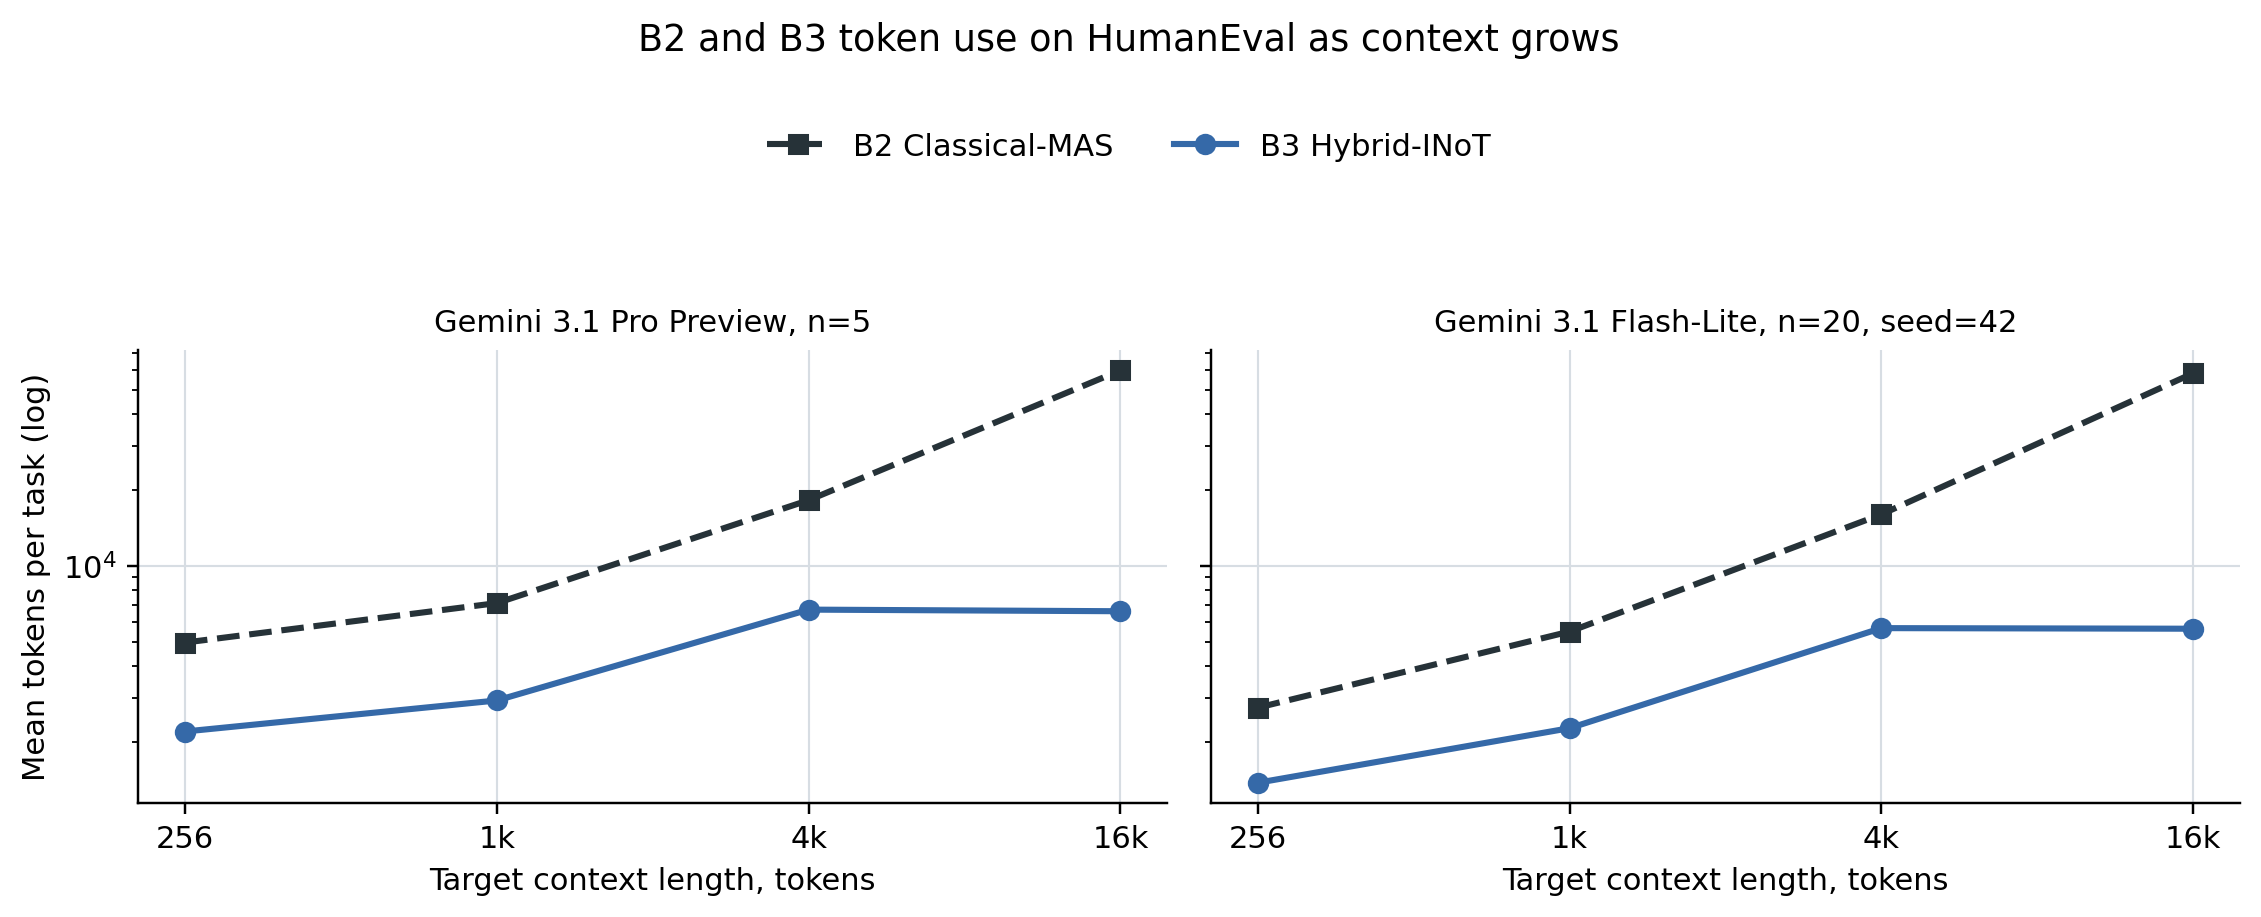
\includegraphics[width=\textwidth]{figures/generated/e3_humaneval_replication_en.png}
\Description{Mean total tokens per task for B2 Classical-MAS and B3 Hybrid-INoT across context lengths, shown separately for the Pro pilot and Flash-Lite replication.}
\caption{Mean total tokens per task. Dashed squares denote B2 Classical-MAS; solid circles denote B3 Hybrid-INoT. The $y$ axis is logarithmic. Left: retained Pro pilot ($n=5$ per point); right: Flash-Lite replication ($n=20$, seed 42).}
\label{fig:e3-replication}
\end{figure}

For Pro at 16,384 target tokens,
\[
S_T=100\left(1-\frac{6608.4}{59631.4}\right)=88.9\%,\qquad
S_C=100\left(1-\frac{0.0294908}{0.1407228}\right)=79.0\%.
\]
Since pass@1 is one, $U_{B2}=1/59631.4=1.677\cdot10^{-5}$ and $U_{B3}=1/6608.4=1.513\cdot10^{-4}$, an aggregate ratio-of-means gain of 802.4\%. Computing the ratio within each task before aggregation gives 805.7\% (95\% bootstrap CI 753.4--850.1\%).

All Pro paired gains are positive, but with five nonzero one-directional pairs the minimum two-sided $p$ is 0.0625; none is significant after correction. In the Flash-Lite run, mean paired gains are 105.5, 144.3, 183.2, and 934.6\%; all CIs exclude zero, and $p=1.91\cdot10^{-6}$ at every context length, surviving Holm correction.

Nevertheless, pass@1${}=1.0$ for both architectures creates a ceiling. There are no discordant pairs, exact McNemar $p=1$, and the sample does not establish non-inferiority within 2 percentage points. Only the token component of H1 is supported. Because B3 dominates at the leftmost grid point, \path{tau_star=256} means left censoring, $\tau^\star\le256$ target tokens, not a point estimate.

\subsection{E2~--- Ablations, critic behavior, and parallelism}\label{subsec:e2}

The Pro ablation pilot contains five tasks. pass@1 is 1.0 for full B3 and variants without compression, critic, or self-check. Paired aggregate-success differences for full B3 against the three variants are $-0.0037$, $-0.0262$, and $0.0000$, with $p=1.0$, $0.5$, and $1.0$; none survives Holm correction. Component token-overhead shares are 36.6\% for compression, 29.7\% for the critic, and 33.8\% for self-check, but these are overhead allocations, not demonstrated independent quality contributions. Only two B0 failures were available for E2b; zero erroneous critic approvals in two cases do not establish critic reliability.

In E2c, mean B2 latency is 19.28~s and B3 latency 9.76~s, a $-49.4\%$ change; the 95\% bootstrap CI for B3$-$B2 is $[-13.05,-6.83]$~s, but the Wilcoxon test gives $p=0.0625$ at $n=5$. A separate deterministic tool microbenchmark shows serial execution to be 148.8\% slower than parallel execution, yet the direct architectural comparison does not show the predicted B3 penalty. H3 is therefore \emph{not supported}; the microbenchmark only confirms a mechanism requiring isolation on real independent-tool tasks. E2d produces seven ranking inversions under weight and $\lambda$ changes, with the no-critic variant ranked first canonically. The composite metric is therefore unstable and retained only as a secondary measure.

\subsection{E4~--- Economic test of the small model}\label{subsec:e4}

Twenty HumanEval cases and twenty approximate SWE-bench Lite cases were run with Gemini~3.1~Pro Preview as the large model and Flash-Lite as the small model. Net margin per task is
\begin{equation}
M=(\rho_0-\rho_1)C_{\mathrm{rerun}}^L-C_{\mathrm{check}}^S.
\label{eq:e4-margin}
\end{equation}

\begin{table}[htbp]
\caption{Small-model profitability test, USD per task}
\label{tab:e4-results}
\centering
\begin{tabular}{@{}lrrrrrc@{}}
\toprule
Dataset & $\rho_0$ & $\rho_1$ & $C_{\mathrm{check}}^S$ & $C_{\mathrm{rerun}}^L$ & $M$ (95\% CI) & H2 \\
\midrule
HumanEval & .35 & .00 & .000060 & .010822 & .003728 [.002042; .007685] & yes \\
SWE-bench Lite* & .75 & .60 & .000122 & .014469 & .002048 [$-.000104$; .004650] & no \\
\bottomrule
\end{tabular}
\end{table}

For HumanEval, $M=(0.35-0)\cdot0.0108224-0.000060025=0.003727815$, and the lower CI bound is positive. The SWE-bench Lite interval crosses zero, so the original H2 requirement for both datasets is not met. The asterisk is essential: the current loader does not run the official containerized SWE-bench harness~\cite{jimenez2023swebench}; it uses code extraction and a \path{check(_)} stub. This result characterizes the harness routing/check procedure, not the ability to resolve real GitHub issues.

\subsection{E6~--- Cross-model sensitivity}\label{subsec:e6}

The retained E6 compares Pro and Flash-Lite on ten controlled cases per architecture--context cell. Three simple function families are repeated (\path{reverse_words}, \path{count_peaks}, and \path{normalize_path}); pass@1 is 1.0 throughout. At contexts 512, 2,048, and 8,192, Flash-Lite cost is 4.8, 6.9, and 9.7\% of Pro cost for B2, and 4.4, 5.4, and 7.0\% for B3 (Fig.~\ref{fig:e6-cost}). Paired $U_{\mathrm{tok}}$ differences are significant ($p=0.001953$, all survive Holm correction), but the quality ceiling prevents generalization to difficult tasks.

\begin{figure}[htbp]
\centering
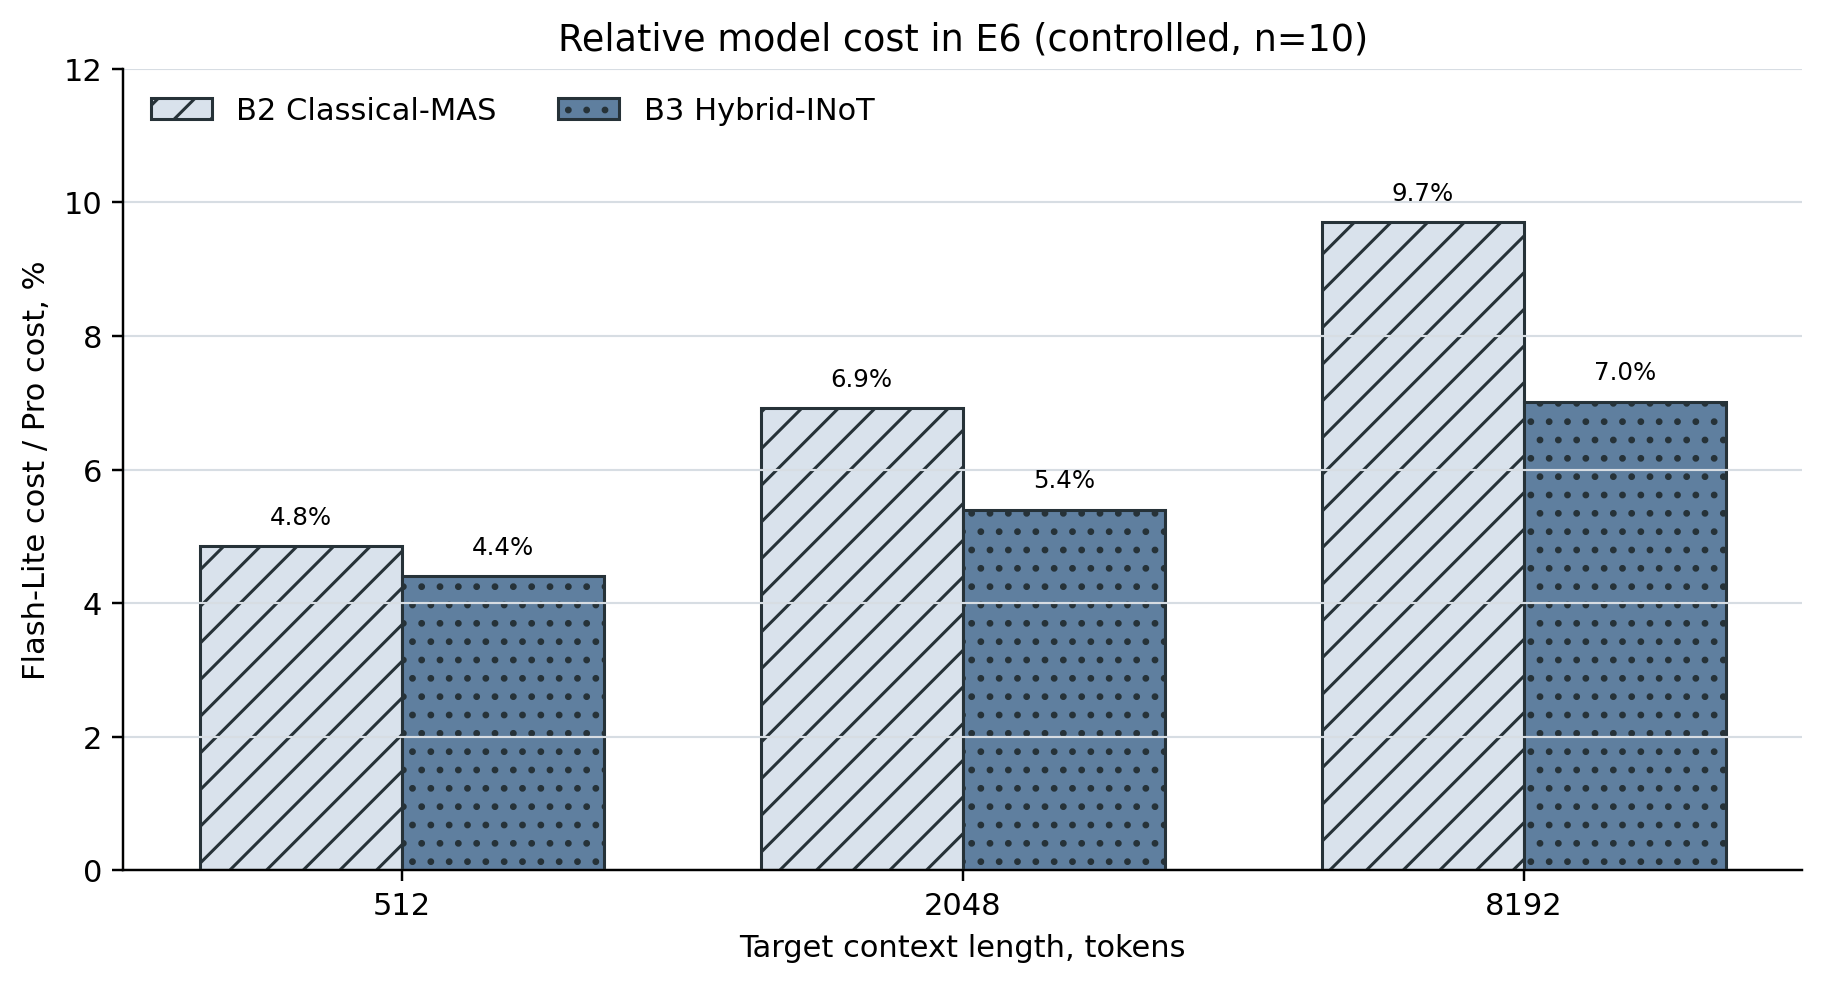
\includegraphics[width=.92\textwidth]{figures/generated/e6_model_cost_ratio_en.png}
\Description{Flash-Lite cost as a percentage of Pro cost across context lengths, shown separately for B2 Classical-MAS and B3 Hybrid-INoT.}
\caption{Mean Gemini~3.1~Flash-Lite cost relative to Gemini~3.1~Pro Preview in controlled E6. Hatching preserves black-and-white readability.}
\label{fig:e6-cost}
\end{figure}

\subsection{E5~--- API-inference cost extrapolation}\label{subsec:e5}

The full TCO experiment was not completed: an additional run hit the provider limit before \textnormal{\texttt{runs.json}} was persisted and is excluded. Instead, we perform an explicitly limited analytical extrapolation from twenty paired Pro E3 cases: five tasks at each of four context lengths with equal weights. For $N$ tasks,
\begin{equation}
\Delta C_{\mathrm{inf}}(N)=N\cdot
\frac{1}{20}\sum_{i=1}^{20}\left(C_{B2,i}-C_{B3,i}\right).
\label{eq:inference-extrapolation}
\end{equation}
The mean difference is \$0.042996 per task; at $N=10,000$, B3 savings are \$429.96, with a 95\% paired-bootstrap CI of \$267.06--\$617.17. Scaling both token prices by $-50,-25,0,+25,+50\%$ gives \$214.98, \$322.47, \$429.96, \$537.45, and \$644.94, respectively (Fig.~\ref{fig:e5-sensitivity}).

\begin{figure}[htbp]
\centering
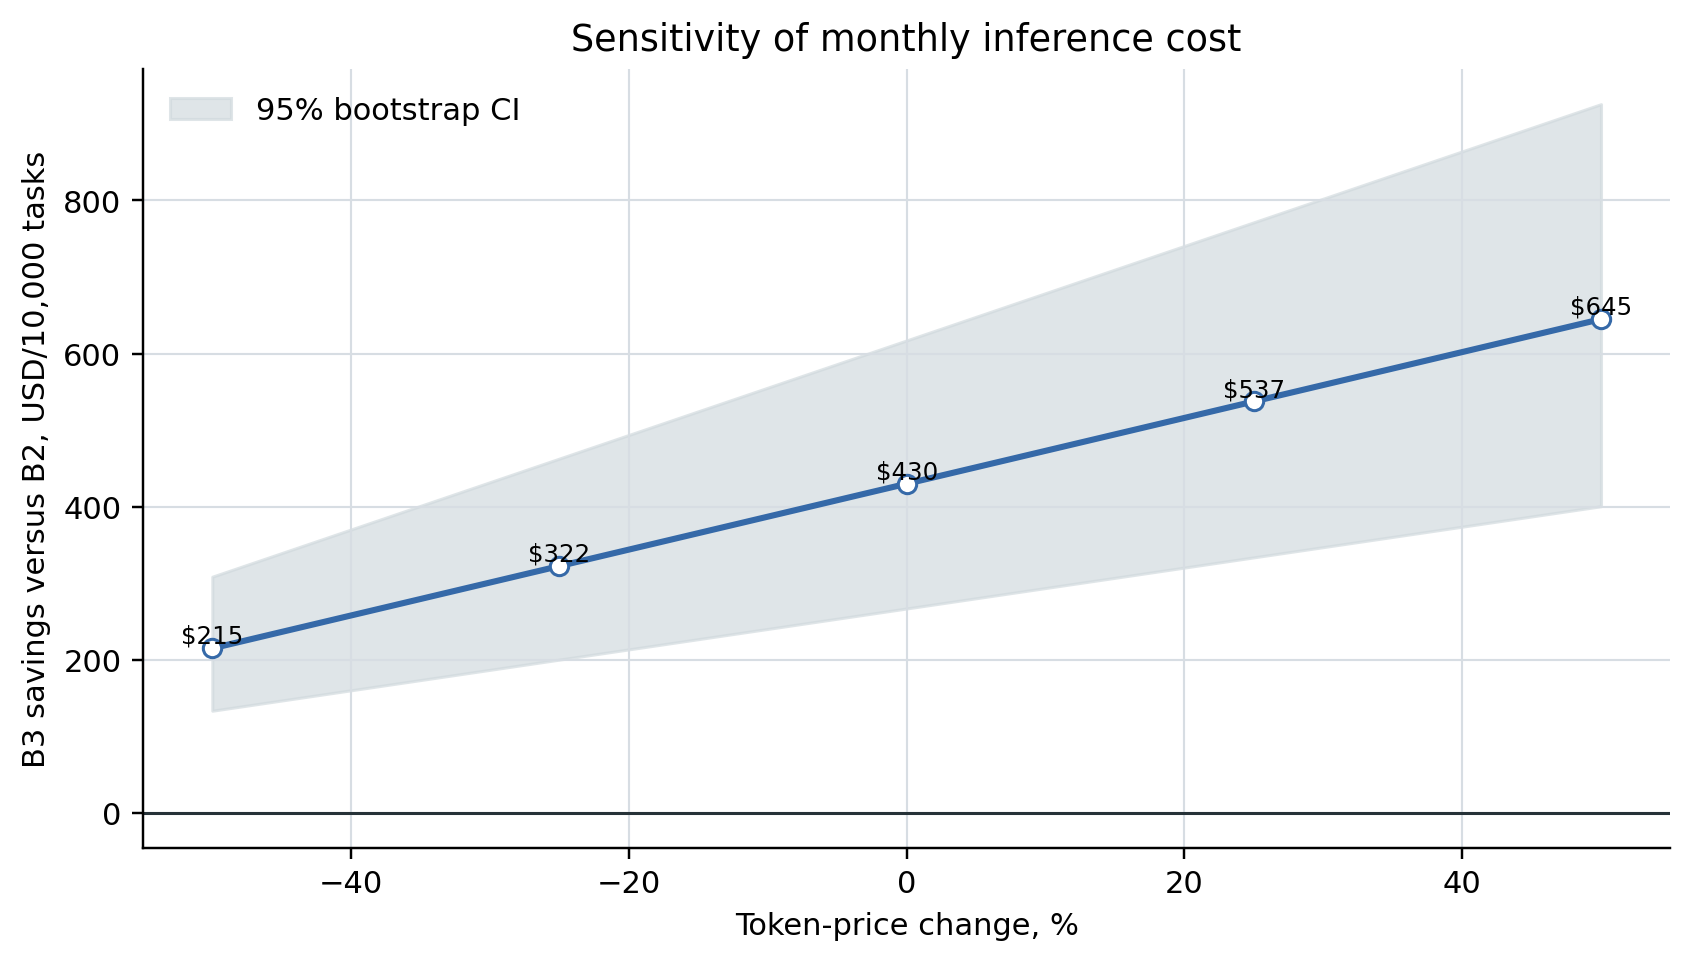
\includegraphics[width=.92\textwidth]{figures/generated/e5_inference_cost_sensitivity_en.png}
\Description{Projected API-inference savings under common token-price multipliers, with a bootstrap interval.}
\caption{Sensitivity of monthly B3 savings versus B2 to a common token-price multiplier: 10,000 tasks and an equal mixture of four context lengths. The band is the 95\% paired-bootstrap CI.}
\label{fig:e5-sensitivity}
\end{figure}

\section{Economic model}\label{sec:tco}

\subsection{Boundary between inference cost and TCO}

\begin{equation}
\mathrm{TCO}_{\text{month}}=C_{\text{inf}}+C_{\text{hw}}+C_{\text{energy}}+C_{\text{storage}}+C_{\text{ops}}.
\label{eq:tco}
\end{equation}

Only external-API $C_{\text{inf}}$ is measured. Hardware, energy, storage, operations, engineering labor, and delay costs are not observed. Thus, E5 supports API-inference savings for the pilot mixture but not $\Delta\mathrm{TCO}<0$.

\subsection{Hypothesis verdicts}

\begin{table}[htbp]
\caption{Original hypotheses versus observed evidence}
\label{tab:hypothesis-verdict}
\centering
\begin{tabularx}{\textwidth}{@{}l l X@{}}
\toprule
Claim & Verdict & Evidence \\
\midrule
H1 & partial & B3 token gain is supported in Flash-Lite; Pro is underpowered, and 2-pp pass@1 non-inferiority is not established. \\
H2 & not supported as stated & Positive CI on HumanEval, but the approximate SWE-bench Lite CI crosses zero. \\
H3 & not supported & The tool microbenchmark favors parallelism, but direct B3 is faster than B2; $n=5$. \\
$\tau^\star$ & not identified & B3 dominates at the left boundary; only $\tau^\star\le256$ target tokens is established. \\
\bottomrule
\end{tabularx}
\end{table}

\section{Limitations and threats to validity}\label{sec:limits}

\begin{enumerate}
\item \textbf{Small, non-random samples.} The first 5 or 20 HumanEval tasks are used rather than a random stratified sample of 164; the new run has one seed.
\item \textbf{Synthetic context.} Long inputs are assembled from other HumanEval tasks rather than repository history. They isolate retransmission cost but not real codebase dependencies.
\item \textbf{Quality ceiling.} B2/B3 and controlled E6 have pass@1${}=1.0$, supporting a resource comparison but not a strong quality test.
\item \textbf{Approximate SWE-bench.} The official container harness is not used, so no claim about real issue resolution is made.
\item \textbf{API drift.} Model names, parameters, usage, latency, and cost are recorded, but aliases do not guarantee immutable weights. Provider-limit failures are excluded.
\item \textbf{Limited answer auditability.} \textnormal{\texttt{runs.json}} records metrics and usage but not complete final solution text.
\item \textbf{Cost is not TCO.} Figure~\ref{fig:e5-sensitivity} covers API inference only; the other terms in~\eqref{eq:tco} are unmeasured.
\item \textbf{Architectural boundaries.} Independent subtasks, process isolation, critic errors, and compression losses may eliminate the B3 advantage. Role text is a computational mechanism, not a faithful explanation of hidden reasoning~\cite{turpin2023unfaithful}.
\end{enumerate}

\section{Directions for further research}\label{sec:agenda}

The next study should remove the identified uncertainty rather than repeat the pilot:
\begin{enumerate}
\item run all 164 HumanEval tasks with at least five seeds and a fixed analysis plan, including a powered non-inferiority test;
\item extend the context grid below 256 tokens to estimate rather than left-censor $\tau^\star$;
\item retain full input/output, prompt hashes, immutable model identifiers, and external-test results per run;
\item replace the approximate SWE-bench path with the official container harness on a random repository sample;
\item repeat E2c with real independent tools under matched models and serial/parallel execution;
\item compare B3 with Self-Refine~\cite{madaan2023selfrefine}, Reflexion~\cite{shinn2023reflexion}, ReAct~\cite{yao2022react}, and SWE-agent~\cite{yang2024sweagent};
\item measure full TCO, including operations, reruns, latency, infrastructure, and storage, under a production context-length distribution.
\end{enumerate}

\section{Conclusion}

Hybrid-INoT is formalized as an intermediate architecture between in-context self-critique and external multi-agent orchestration. The analytical model predicts a growing advantage with shared-context length, and two real API pilots agree with that prediction. In the 20-task Flash-Lite replication, B3 uses 49.6--90.3\% fewer tokens than B2, and paired $U_{\mathrm{tok}}$ gains remain significant after multiple-comparison correction. However, ceiling pass@1 does not establish quality non-inferiority; H2 is supported only on HumanEval; H3 is not supported in the direct pilot; and the \$429.96 per 10,000 tasks estimate covers API inference only. The evidence therefore supports Hybrid-INoT as a promising mechanism for reducing repeated long-context transmission, while quality, the applicability threshold, and full economic impact require a powered evaluation on real repositories.


\section*{Data Availability}
An anonymous replication package is available at \url{https://anonymous.4open.science/r/hybrid-inot-july-2026/}. The downloadable archive, \texttt{hybrid-inot-july-2026-anonymous.zip}, contains the frozen research harness, configurations, recorded metrics and usage, and scripts and source data for the reported tables and figures. The records do not include complete generated solution text; this limits answer-level auditing. The package supports inspection and offline analysis of retained results; rerunning hosted models may require an API account and may be affected by model drift. The replication materials will be made publicly available upon acceptance.
\nocite{austin2021mbpp,goncalves2011,ko2007,parnin2011}
\bibliographystyle{ACM-Reference-Format}
\bibliography{references}
\end{document}
